\documentclass[titlepage, letterpaper, fleqn]{article}
\usepackage[utf8]{inputenc}
\usepackage{fancyhdr} % fancy headers, of course!
\usepackage{amsmath} % what do you think?
\usepackage{amsthm} % theorems!
\usepackage{extramarks} % more cute things
\usepackage{enumitem} % i'm not sure...
\usepackage{multicol} % multicolumn...?
\usepackage{amssymb} % more symbols
\usepackage{booktabs} % cool looking tables
\usepackage{tikz} %venn and shizzle
\usepackage{tikz-qtree-compat} %tableaux
\usepackage{lipsum} %lorem ipsum dolor sit amet f u
\usepackage{mathrsfs} %math script for calligraphic scripting, I GUESS

\topmargin=-0.45in
\evensidemargin=0in
\oddsidemargin=0in
\textwidth=6.5in
\textheight=9.0in
\headsep=0.25in


%
% You should change this things~
%

\newcommand{\mahteacher}{Dr. Viacheslav Kalashnikov}
\newcommand{\mahclass}{Applied Mathematics}
\newcommand{\mahtitle}{Topic II - Activity 8}
\newcommand{\mahdate}{September 28, 2016}
\newcommand{\spacepls}{\vspace{5mm}}
\newcommand{\numberthis}{\addtocounter{equation}{1}\text{\theequation}}
\renewcommand\qedsymbol{\(\blacksquare\)}

%
% Header markings
%

\pagestyle{fancy}
\lhead{1170065 - Xavier Sánchez}
\chead{}
\rhead{}
\lfoot{}
\rfoot{}


\renewcommand\headrulewidth{0.4pt}
\renewcommand\footrulewidth{0.4pt}

\setlength\parindent{0pt}


%
% Create Problem Sections (stolen directly from jdavis/latex-homework-template @ github!)
%

\newcommand{\enterProblemHeader}[1]{
\nobreak\extramarks{}{Problem \arabic{#1} continued on next page\ldots}\nobreak{}
\nobreak\extramarks{Problem \arabic{#1} (continued)}{Problem \arabic{#1} continued on next page\ldots}\nobreak{}
}

\newcommand{\exitProblemHeader}[1]{
\nobreak\extramarks{Problem \arabic{#1} (continued)}{Problem \arabic{#1} continued on next page\ldots}\nobreak{}
\stepcounter{#1}
\nobreak\extramarks{Problem \arabic{#1}}{}\nobreak{}
}

\setcounter{secnumdepth}{0}
\newcounter{partCounter}
\newcounter{homeworkProblemCounter}
\setcounter{homeworkProblemCounter}{1}
\nobreak\extramarks{Exercise \arabic{homeworkProblemCounter}}{}\nobreak{}

% Alias for the Solution section header
\newcommand{\solution}{\textbf{\Large Solution}}

%Alias for the new step section
\newcommand{\steppy}[1]{\textbf{\large #1}}

%
% Homework Problem Environment
%
% This environment takes an optional argument. When given, it will adjust the
% problem counter. This is useful for when the problems given for your
% assignment aren't sequential. See the last 3 problems of this template for an
% example.
%
\newenvironment{homeworkProblem}[1][-1]{
\ifnum#1>0
\setcounter{homeworkProblemCounter}{#1}
\fi
\section{Exercise \arabic{homeworkProblemCounter}}
\setcounter{partCounter}{1}
\enterProblemHeader{homeworkProblemCounter}
}{
\exitProblemHeader{homeworkProblemCounter}
}

%
% Venn diagrams defs
%

% \def\firstcircle{(0,0) circle (1.5cm)}
% \def\secondcircle{(0:2cm) circle (1.5cm)}
% \colorlet{circle edge}{blue!50}
% \colorlet{circle area}{blue!20}

% \tikzset{filled/.style={fill=circle area, draw=circle edge, thick},
%     outline/.style={draw=circle edge, thick}}

%
% My actual info
%

\title{
\vspace{1in}
\textbf{Tecnológico de Monterrey} \\
\vspace{0.5in}
\textmd{\mahclass} \\
\large{\textit{\mahteacher}} \\
\vspace{0.5in}
\textsc{\mahtitle}\\
\textsc{2.2.1 Propositional Logic}\\
\textsc{2.2.2 Propositional Logic}\\
\textsc{2.2.3 Propositional Logic}\\
%\textsc{2.2.4 Propositional Logic}
\author{01170065  - MIT \\
Xavier Fernando Cuauhtémoc Sánchez Díaz \\
\texttt{xavier.sanchezdz@gmail.com}}
\date{\mahdate}
}

\begin{document}

\begin{titlepage}
\maketitle
\end{titlepage}

%
% Actual document starts here~
%

\section{Exercise 2.2.1}

{\large \textbf{a)} Prove \((A \implies B) \implies (\neg B \implies \neg A)\) in \(\mathscr{G}\).}

The semantic tableau for the converse of \((A \implies B) \implies (\neg B \implies \neg A)\) is as follows:

\spacepls

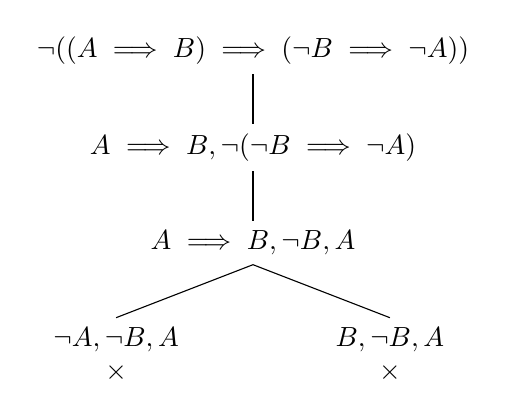
\begin{tikzpicture}
\tikzset{every tree node/.style={align=center,anchor=north}}
\tikzset{sibling distance=50pt}
\tikzset{level distance=35pt}
\tikzset{grow'=down}
\Tree [.{$\neg((A \implies B) \implies (\neg B \implies \neg A))$} 
[.{$A \implies B, \neg (\neg B \implies \neg A)$} 
[.{$A \implies B, \neg B, A$} 
[.{$B, \neg B, A$}\\{$\times$} ] 
[.{$\neg A, \neg B, A$}\\{$\times$} ] ] ] ]
\end{tikzpicture}

\spacepls

\begin{proof}
\begin{align}
& A, B, \neg A & \text{Axiom} \label{ax1a}
\\ & \neg B, B, \neg A & \text{Axiom} \label{ax2a}
\\ & \neg(A \implies B), B, \neg A & \text{$\beta$-rule on \ref{ax1a} and \ref{ax2a}} \label{step3a}
\\ & \neg(A \implies B), \neg B \implies \neg A & \text{$\alpha$-rule on \ref{step3a}} \label{step4a}
\\ & (A \implies B) \implies (\neg B \implies \neg A) & \text{$\alpha$-rule on \ref{step4a}}
\end{align}
\end{proof}

{\large \textbf{b)} Prove \((A \implies B) \implies ((\neg A \implies B)\implies B)\) in \(\mathscr{G}\).}

The semantic tableau for the converse of \((A \implies B) \implies ((\neg A \implies B)\implies B)\) is as follows:

\spacepls

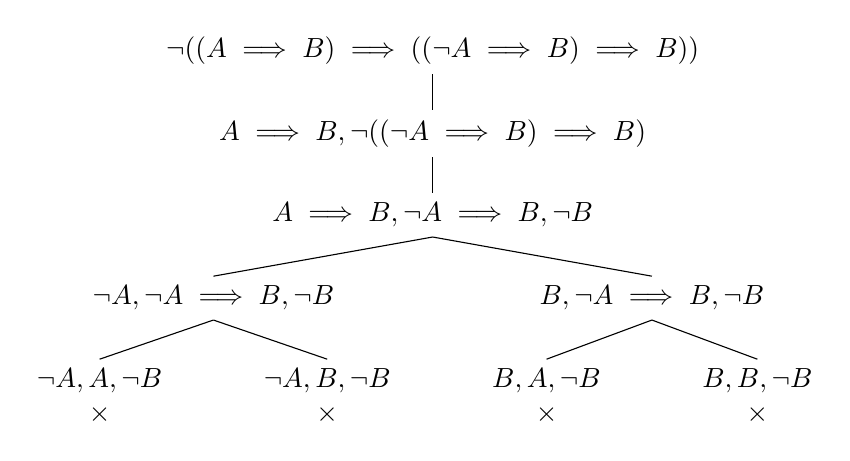
\begin{tikzpicture}
\tikzset{every tree node/.style={align=center,anchor=north}}
\tikzset{sibling distance=30pt}
\tikzset{grow'=down}
\Tree [.{$\neg ((A \implies B) \implies ((\neg A \implies B) \implies B))$} 
      [.{$A \implies B, \neg ((\neg A \implies B) \implies B)$} 
      [.{$A \implies B, \neg A \implies B, \neg B$} 
      [.{$B, \neg A \implies B, \neg B$} {$B, B, \neg B$\\{$\times$}} {$B, A, \neg B$\\{$\times$}} ] 
      [.{$\neg A, \neg A \implies B, \neg B$} {$\neg A, B, \neg B$\\{$\times$}} {$\neg A, A, \neg B$\\{$\times$}} ] ] ] ]
\end{tikzpicture}

\begin{proof}
\begin{align}
& A, \neg A, B & \text{Axiom} \label{ax1b}
\\ & A \neg B, B & \text{Axiom} \label{ax2b}
\\ & \neg B, \neg A, B & \text{Axiom} \label{ax3b}
\\ & \neg B, \neg B, B & \text{Axiom} \label{ax4b}
\\ & A, \neg(\neg A \implies B), B & \text{$\beta$-rule on \ref{ax1b}, \ref{ax2b}} \label{step5b}
\\ & \neg B, \neg(\neg A \implies B), B & \text{$\beta$-rule on \ref{ax3b}, \ref{ax4b}} \label{step6b}
\\ & \neg (A \implies B), \neg (\neg A \implies B), B & \text{$\beta$-rule on \ref{step5b}, \ref{step6b}} \label{step7b}
\\ & \neg (A \implies B), (\neg A \implies B) \implies B & \text{$\alpha$-rule on \ref{step7b}} \label{step8b}
\\ & (A \implies B) \implies ((\neg A \implies B)\implies B) & \text{$\alpha$-rule on \ref{step8b}}
\end{align}
\end{proof}

{\large \textbf{c)} Prove \(((A \implies B) \implies A) \implies A\) in \(\mathscr{G}\).}

The semantic tableau for the converse of \(((A \implies B) \implies A) \implies A\) is as follows:

\spacepls

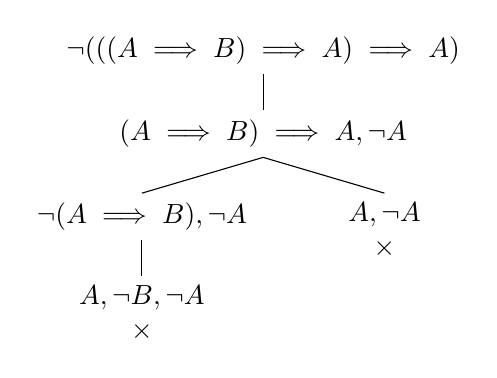
\begin{tikzpicture}
\tikzset{every tree node/.style={align=center,anchor=north}}
\tikzset{sibling distance=30pt}
\tikzset{grow'=down}
\Tree [.{$\neg (((A \implies B) \implies A) \implies A)$} 
[.{$(A \implies B) \implies A, \neg A$} 
{$A, \neg A$}\\{$\times$} 
[.{$\neg(A \implies B), \neg A$} 
{$A, \neg B, \neg A$}\\{$\times$} ] ] ]
\end{tikzpicture}

\begin{proof}
\begin{align}
& \neg A, B, A & \text{Axiom} \label{ax1c}
\\ & \neg A, A & \text{Axiom} \label{ax2c}
\\ & A \implies B, A & \text{$\alpha$-rule on \ref{ax1c}} \label{step3c}
\\ & \neg((A \implies B) \implies A), A & \text{$\beta$-rule on \ref{step3c}} \label{step4c}
\\ & ((A \implies B) \implies A) \implies A & \text{$\alpha$-rule on \ref{step4c}}
\end{align}
\end{proof}

\section{Exercise 2.2.2}

{\large \textbf{a)} Prove the derived rule \textit{modus tollens}: \(\dfrac{\vdash \neg B \, \, \, \, \, \, \, \vdash A \implies B}{\vdash \neg A}\).}

\spacepls

To show that \textit{modus tollens} is a valid rule of inference, proving the converse should suffice:

\begin{proof}
\begin{align*}
& \neg((\neg B \wedge (A \implies B)) \implies \neg A) = & \tag*{Converse}
\\ & = (\neg B \wedge (A \implies B)) \wedge A & \tag*{Material implication \& de Morgan}
\\ & = \neg B \wedge (\neg A \vee B) \wedge A & \tag*{Material implication}
\\ & = (A \wedge \neg B \wedge \neg A) \vee (A \wedge \neg B \wedge B) & \tag*{$\wedge$ is commutative, $\wedge$ distributes over $\vee$}
\end{align*}

Since both \(A \wedge \neg B \wedge \neg A\) and \(A \wedge \neg B \wedge B\) are contradictions, this converse is unsatisfiable.

Therefore, \textit{modus tollens} is a valid inference rule.
\end{proof}

\section{Exercise 2.2.3}

{\large \textbf{a)} Prove \(\vdash (A \implies B) \vee (B \implies A)\) in \(\mathscr{H}\):}

\begin{proof}
\begin{align}
& \{\neg (A \implies B), B \} \vdash B & \text{Assumption} \label{ex3:a1}
\\ & \{\neg (A \implies B), B \} \vdash \neg (A \implies B) & \text{Assumption} \label{ex3:a2}
\\ & \{\neg (A \implies B), B \} \vdash \neg(A \implies B) \implies (A \wedge \neg B) & \text{Definition of \(\wedge\)} \label{ex3:step3}
\\ & \{\neg (A \implies B), B \} \vdash (A \wedge \neg B) & \text{MP \ref{ex3:a2}, \ref{ex3:step3}} \label{ex3:step4}
\\ & \{\neg (A \implies B), B \} \vdash (A \wedge \neg B) \implies A & \text{B is assumed on \ref{ex3:a1}} \label{ex3:step5}
\\ & \{\neg (A \implies B), B \} \vdash A & \text{MP \ref{ex3:step4}, \ref{ex3:step5}} \label{ex3:step6}
\\ & \{\neg (A \implies B)\} \vdash B \implies A & \text{Deduction \ref{ex3:step6}} \label{ex3:step7}
\\ & \vdash \neg (A \implies B) \implies (B \implies A) & \text{Deduction \ref{ex3:step7}}
\\ & \vdash (A \implies B) \vee (B \implies A) & \text{Definition of \(\vee\)}
\end{align}
\end{proof}

% I should finish this
% \section{2.2.4}

% {\large \textbf{a)} Prove \((A \implies B) \implies ((\neg A \implies B)\implies B)\) in \(\mathscr{H}\).}

% \begin{proof}
% aa
% \end{proof}

% {\large \textbf{c)} Prove \(((A \implies B) \implies A) \implies A\) in \(\mathscr{H}\).}

% \begin{proof}
% aa
% \end{proof}

\end{document}